\documentclass{article}
\usepackage[utf8]{inputenc}
\usepackage[hidelinks]{hyperref}
\usepackage{xcolor}
\usepackage[T1]{fontenc}
\usepackage{listings}
\usepackage{xcolor}
\usepackage{graphicx}
\usepackage[a4paper, left = 3cm, right = 3cm, top =2cm]{geometry}
\definecolor{codegreen}{rgb}{0,0.6,0}
\definecolor{codegray}{rgb}{0.5,0.5,0.5}
\definecolor{codepurple}{rgb}{0.58,0,0.82}
\definecolor{backcolour}{rgb}{0.95,0.95,0.92}
\definecolor{redflag}{rgb}{0.266,0,0}
\definecolor{blueflagg}{rgb}{0,87,214}
\definecolor{darkblueflag}{rgb}{0,33,66}
\definecolor{customGreen}{HTML}{228B22}
\lstdefinestyle{mystyle}{
    backgroundcolor=\color{backcolour},   
    commentstyle=\color{codegreen},
    keywordstyle=\color{magenta},
    numberstyle=\tiny\color{codegray},
    stringstyle=\color{codepurple},
    basicstyle=\ttfamily\footnotesize,
    breakatwhitespace=false,         
    breaklines=true,                 
    captionpos=b,                    
    keepspaces=true,                 
    numbers=left,                    
    numbersep=5pt,                  
    showspaces=false,                
    showstringspaces=false,
    showtabs=false,                  
    tabsize=2
}
\lstset{keepspaces=true, style=mystyle}

\begin{document}
\begin{titlepage}
    \begin{center}
    {
\includegraphics[width=0.15\textwidth]{img/matcom.jpg}\par}
    \vspace{0.1cm}
    {\bfseries\LARGE Ciencia de Datos \par}
    \vspace{0.2cm}
    {\scshape\Large  Facultad de Matemática y Computación\par}
    \vspace{0.6cm}
    {\scshape\Huge{{\textbf{Introducción a la Ciencia de Datos \\ Proyecto Final}} \par}
    \vspace{0.2cm}
    {\itshape\Large {\large{\textit{Procesos migratorios en Cienfuegos}}} \par}
    \vspace{0.8cm}
    {\large Autor: \\ \normalsize{Luis Ernesto Serras Rimada} \par}
    \vspace{0.5cm}
    {
\includegraphics[width=0.85\textwidth]{img/perla.png}}
    \end{center}
\end{titlepage}
\newpage
\section{Introducción}
La búsqueda de mejores oportunidades de empleo y educación es un impulso fundamental que motiva a las personas a migrar, tanto a nivel interno como externo. Este fenómeno refleja no solo la aspiración individual de alcanzar una vida más digna y satisfactoria, sino también un contexto socioeconómico que, en muchos casos, limita el desarrollo personal y profesional en sus lugares de origen. La decisión de emprender este camino, aunque a menudo dolorosa y compleja, simboliza la lucha por la superación y el deseo de construir un futuro mejor. Al mismo tiempo, pone de manifiesto las disparidades entre regiones, donde lugares como \textcolor{orange}{La Habana} ofrecen un abanico más amplio de oportunidades comparado con provincias como \textcolor{blue}{Cienfuegos}. En última instancia, este deseo de progreso se convierte en una fuerza dinámica que puede transformar realidades, tanto para los individuos como para las comunidades a las que pertenecen.


\section{Desarrollo}
\subsection{Recopilación y procesamiento de los datos}
La fuente principal de los datos manejados fueron las series estadísticas y anuarios de la \textcolor{blue}{Oficina Nacional de Estadosisticas e Información (ONEI)}. Las series estadísticas empleadas en formato .xls (llevados a formato csv) fueron reacomodados a mano mayormente para luego limpiarlos haciendo uso del modulo \textcolor{green}{csv} de \textcolor{blue}{Python}.\\ 
El análisis en su totalidad fue realizado manejando datos procesados y cargados unicamente desde la manipulación directa de los \textcolor{green}{csv} por medio del módulo de \textcolor{blue}{pandas}.

\begin{lstlisting}[language=Python, caption=Funcion para la limpieza de los csv (eliminar espacios adicionales)]
# Function to skip initial space on csv's files
def skipinitalspace_csv(path:str):
    from csv import reader, writer
    data = []
    with open(path, "r") as f:
        reader = reader(f, skipinitialspace=True)
        for i in reader:
            data.append(i)
    with open(path, 'w') as f:
        writer = writer(f)
        writer.writerows(data)
\end{lstlisting}


\begin{lstlisting}[language=Python, caption=Funcion utilizada para parte del procesamiento de algunos datos]
    def migratory_movements(df: pd.core.frame.DataFrame, type:str="prov") -> list[pd.core.frame.DataFrame]:
    #Funcion para el procesamiento de los datos
    if type == "prov":
        year2012, year2013, year2014, year2015, year2016, year2017, year2018, year2019, year2020, year2021, year2022 = 0,0,0,0,0,0,0,0,0,0,0
        dfs = [year2012, year2013, year2014, year2015, year2016, year2017, year2018, year2019, year2020, year2021, year2022]
        i = 1
        for index in range(len(dfs)):
            j = i + 49
            dfs[index] = df.iloc[i:j:3,:]
            dfs[index].set_index("PROCEDENCIA/DESTINO", inplace=True)
            dfs[index].index.name='Anno'
            i = j + 3
    elif type == "mun":
        year2019, year2020, year2021, year2022 = 0,0,0,0
        dfs = [year2019, year2020, year2021, year2022]
        i = 1
        for index in range(len(dfs)):
            j = i + 8
            dfs[index] = df.iloc[i:j,:]
            dfs[index].set_index("ANNOS", inplace=True)
            dfs[index].index.name='Anno'
            i = j + 1
    elif type == "etc":
        prov1, prov2, prov3, prov4, prov5, prov6, prov7, prov8, prov9, prov10, prov11, prov12, prov13, prov14, prov15 = 0,0,0,0,0,0,0,0,0,0,0,0,0,0,0
        dfs = [prov1, prov2, prov3, prov4, prov5, prov6, prov7, prov8, prov9, prov10, prov11, prov12, prov13, prov14, prov15]
        i = 1
        for index in range(len(dfs)):
            j = i + 12
            dfs[index] = df.iloc[i:j,:]
            dfs[index].set_index("PROVINCIAS/ANNOS", inplace=True)
            dfs[index].index.name='Anno'
            i = j + 1                    
    return dfs
\end{lstlisting}

Para manejar los datos se hizo uso de la historia de \textcolor{blue}{Perla}, una joven cienfueguera que (como parte de su desarollo como estudiante de 12mo grado de Preuniversitario, situación familiar y residencial) se enfrenta a los dilemas que se desean exponer, y de esa forma según se avanza en la historia se van presentando los datos visualizandolos de forma natural e interactiva siguiendo la historia.\\\\

Y finalmente para el mapa de densidad se trabajó con la fuente del repositorio de \textcolor{orange}{geojsons} de Cuba de \textcolor{blue}{Yudivián Almeida}. A partir de ellos, además de establecer 
las divisiones del territorio nacional y por provincias, se fueron agregando los valores que se quisieron representar en el mapa y en el tooltip por medio del siguiente script:
\begin{lstlisting}[language=Python, caption=Script para agregar valores al geojson]
    import json 
    import pandas as pd
    '''
    Script para agregar los valores que se mostrarian en el tooltip del mapa al geojson
    '''
    with open("app/data/geojsons/cuba.geojson") as json_file:
        data = json.load(json_file)
    path = "app/data/csv/Movimiento migratorio interno por sexos y provincias.csv"
    
    def skipinitalspace_csv(path:str):
        from csv import reader, writer
        data = []
        with open(path, "r") as f:
            reader = reader(f, skipinitialspace=True)
            for i in reader:
                data.append(i)
        with open(path, 'w') as f:
            writer = writer(f)
            writer.writerows(data)
    skipinitalspace_csv(path)
    
    df = pd.read_csv(path)
    def migratory_movements(df: pd.core.frame.DataFrame) -> list[pd.core.frame.DataFrame]:
        year2012, year2013, year2014, year2015, year2016, year2017, year2018, year2019, year2020, year2021, year2022 = 0,0,0,0,0,0,0,0,0,0,0
        dfs = [year2012, year2013, year2014, year2015, year2016, year2017, year2018, year2019, year2020, year2021, year2022]
        i = 1
        for index in range(len(dfs)):
            j = i + 49
            dfs[index] = df.iloc[i:j:3,:]
            dfs[index].set_index("PROCEDENCIA/DESTINO", inplace=True)
            dfs[index].index.name=None
            i = j + 3
        return dfs
    
    df = migratory_movements(df)
    years = [x for x in range(2012,2023)] #Ordederd list of years
    provincias = list(df[0].columns)[1:]
    
    #Provincias en el orden que aparece en la estructura del GeoJson
    lista_prov = ["La Habana","Matanzas","Cienfuegos","Sancti Spiritus","Las Tunas","Holguin","Granma","Santiago de Cuba","Isla de la Juventud"
                  ,"Camaguey","Ciego de Avila","Villa Clara","Guantanamo","Pinar del Rio","Artemisa","Mayabeque"] 
    
    index = 0
    n = list(df[0].index)
    for year in years:    
        for index, prov in enumerate(lista_prov):
            values = list(df[years.index(year)].iloc[:,n.index(prov)])[1:]
            for k, j in list(zip(provincias,values)):
                data["features"][index]["properties"][f"{k}{year}"] = j    
    try:
        with open("app/data/geojsons/cuba.geojson", 'w') as archivo_json:
            json.dump(data, archivo_json, indent=4)
            print("GeoJson Actualizado de forma exitosa")
    except Exception as e:
        print(f"Error al procesar el GeoJson: {e}") 
\end{lstlisting}

\subsection{Visualizaciones}
Como parte principal de este análisis se procede a visualizar los datos recopilados para valorar su comportamiento.

\subsubsection{Población}
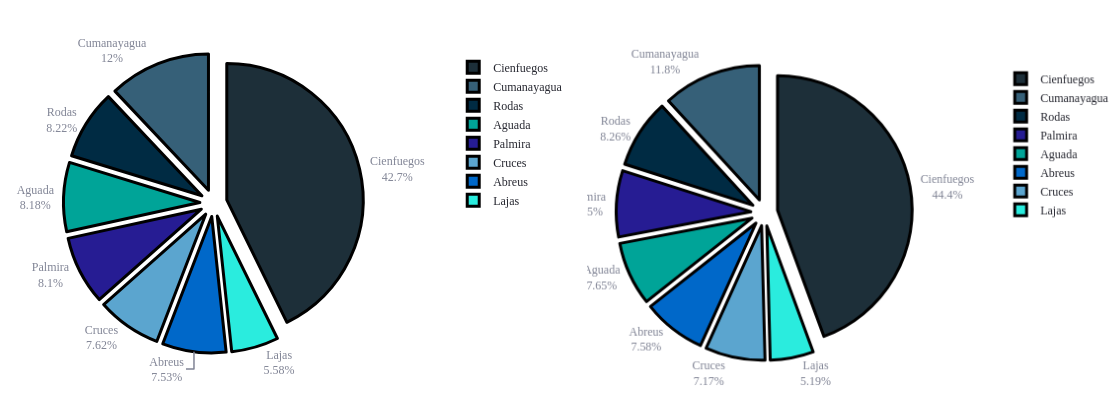
\includegraphics[width=1.0\textwidth]{img/fig1.png}
Se desea partir de analizar la distribución territorial del municipio que se quiere estudiar, por lo que con esta representación \textcolor{blue}{(dividida por edad no laboral a la izquierda y edad laboral a la derecha)} se descubre el predominio de densidad del municipio cabecera con respecto al resto reflejando un claro desblanace de gestión de recursos municipales.

\subsubsection{Educación superior}
Siguiendo el devenir de la narrativa expuesta se introduce una observación referente al número de matriculas iniciales y graduados en comparación para cada año en \textcolor{blue}{Cienfuegos} de la educación superior (la cual cabe resaltar que sólo cuenta con 3 universidades y todas en el municipio cabecera)\\\\
Alcanzando a reflejarse el poco volumen de matrículas y la enorme diferencia referente al número de graduados para cada año en una provincia cuyas unicas instituciones de educación superior radican en la cabecera, por lo que claramente las características del entorno para el escenario de quedarse en su provincia natal van esfumando toda idea o interés por seguir en ese sitio.
En medio de esta problemática nace la problemática de la toma de una decisión crucial para la chica, estudiar en la capital lo que quiere o conformarse con lo que su municipio le ofrece, cada alternativa con sus características particulares descritas.
\begin{center}
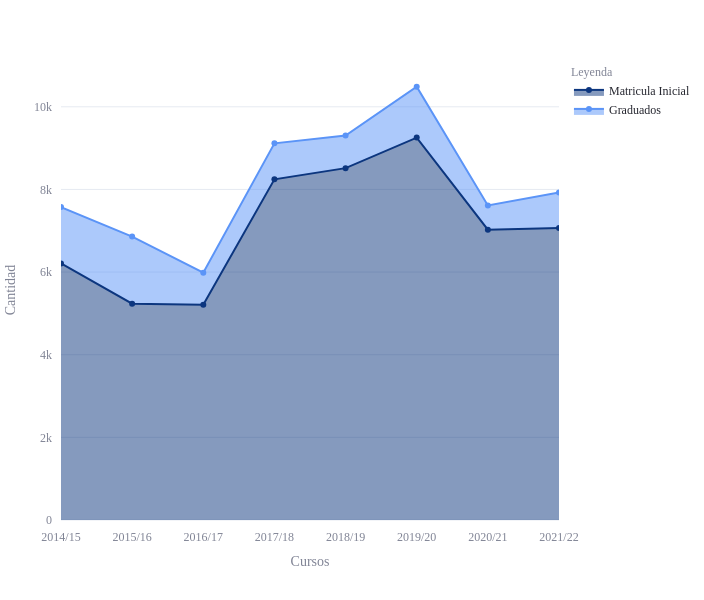
\includegraphics[width=0.7\textwidth]{img/fig2.png}
\end{center}
Luego, acto seguido a introducir al personaje del padre de la joven con su acción de migrar en el pasado, se procede a analizar los procesos migratorios del territorio cubano y del municipio en profundidad.
\subsubsection{Movimientos migratorios}
Dentro de este apartado se plantea estudiar los movimientos migratorios en la isla por provincias para así evaluar de forma nacional y realizar comparaciones aprovechando la interactividad del recurso presentado en un mapa de densidad.
\begin{center}
    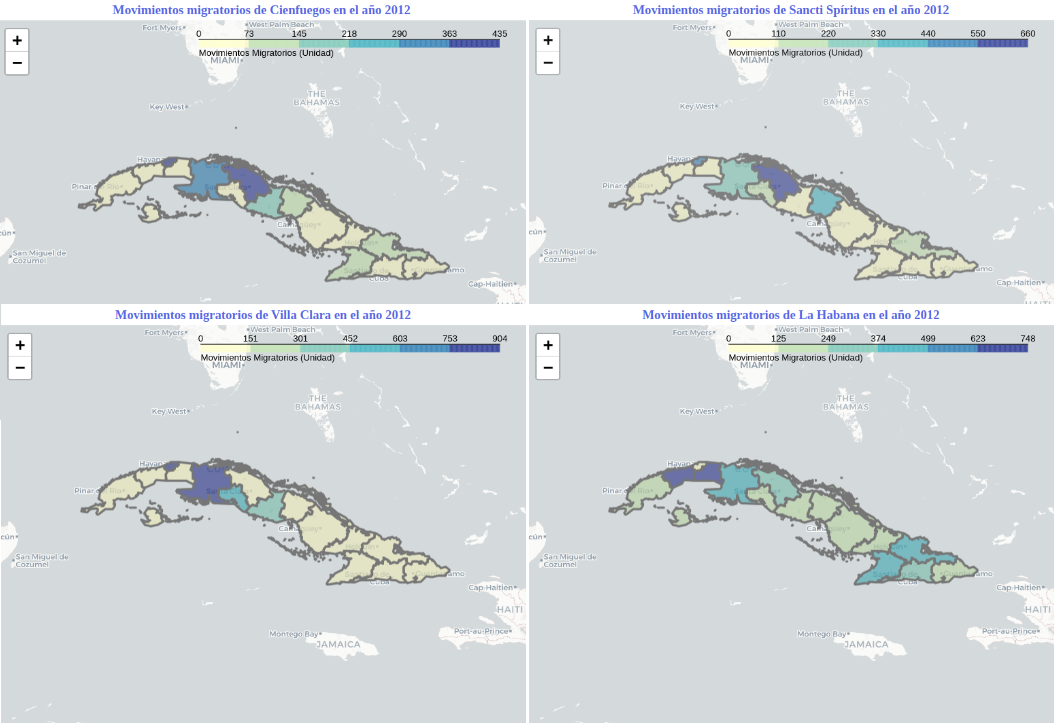
\includegraphics[width=0.9\textwidth]{img/fig3.png}
\end{center}
\newpage
Se observa que los flujos más significativos se dirigen principalmente hacia las provincias de \textcolor{orange}{Villa Clara}, \textcolor{orange}{Matanzas} y \textcolor{orange}{La Habana}. Por otro lado hacia \textcolor{blue}{Cienfuegos} se tiene, en muy pocos volumenes, a provincias como \textcolor{orange}{Sancti Spírictus}, \textcolor{orange}{La Habana}, \textcolor{orange}{Matanzas} y en mayores valores con \textcolor{blue}{532 unidades para el año 2012} se encuentra \textcolor{orange}{Villa Clara} como principal origen.
\subsubsection{Saldo y tasa de migración}
Luego, se aprecia que a diferencia de otras regiones de Cuba, \textcolor{blue}{Cienfuegos} presenta una notable estabilidad en su saldo migratorio interno, lo que significa que los movimientos migratorios interprovinciales se equilibran de manera más favorable en comparación con el típico saldo negativo que caracteriza al país en su conjunto de forma general.
\begin{center}
    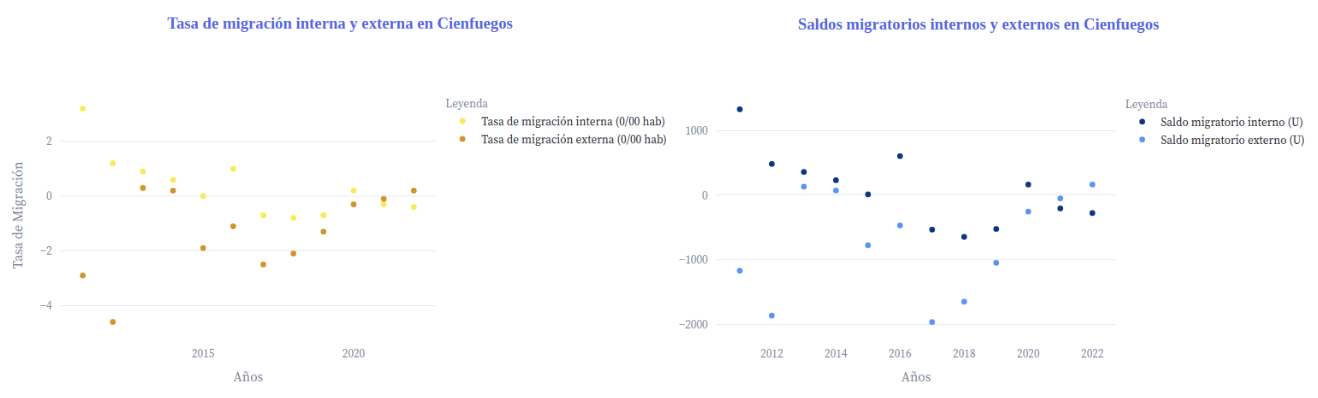
\includegraphics[width=1.0\textwidth]{img/fig4.png}
\end{center}
Sin embargo, al analizar la dinámica migratoria a nivel municipal, se evidencia una tendencia significativa hacia el municipio de cabecera, \textcolor{blue}{Cienfuegos}, dominando la densidad poblacional del municipio agrupando a más del 40\% de la población residente. Este dato revela que, a pesar de la estabilidad general de \textcolor{blue}{Cienfuegos}, existe un posible desbalance intermunicipal que podría estar impulsado por la búsqueda de mejores oportunidades laborales, educación y calidad de vida\\\\
Además, al considerar los diferentes tipos de saldos migratorios, se concluye que, en términos generales, el saldo externo es el que se lleva la delantera con valores negativos (excluyendo la diferencia de saldo interno del municipio \textcolor{blue}{Cienfuegos}). Esto sugiere que, si bien \textcolor{blue}{Cienfuegos} mantiene un equilibrio interno más sólido, la migración hacia el extranjero también juega un papel crucial en la configuración de su demografía y, por ende, en el futuro desarrollo de la región.
\begin{center}
    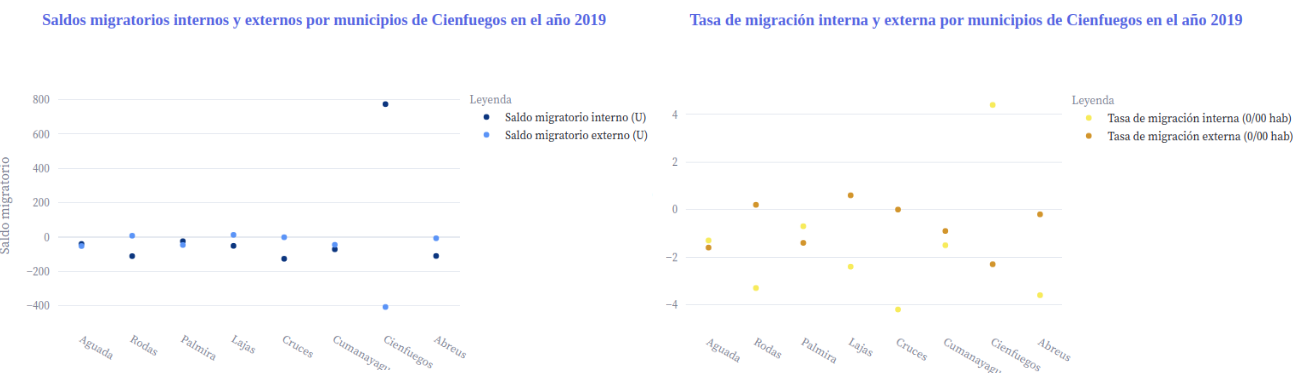
\includegraphics[width=1.0\textwidth]{img/fig5.png}
\end{center}
\subsubsection{Salario medio y empleos}
En el ámbito de las oportunidades laborales (desarrollando en base al contexto de la narración en busca de intentar explicar o hallarle un motor a de Andrés, el padre de Perla, de abandonar a su familia), se tiene a \textcolor{orange}{La Habana} se posiciona como un imán para quienes buscan una mejor calidad de trabajo y un nivel de vida más elevado. En comparación con \textcolor{blue}{Cienfuegos}, la capital ofrece mayores posibilidades de empleo, con una variedad más amplia de sectores y empresas que garantizan salarios medios más altos. Además, en \textcolor{orange}{La Habana}, es más común acceder a créditos y a una gama de servicios que facilitan el desarrollo personal y profesional, lo que atrae a muchos migrantes de otras provincias en busca de un futuro más prometedor.\\
Entonces se decide evaluar (con el fin de minimizar el número de líneas, excluyendo las que no nos aporten al análisis siguiendo el hilo de desarrollo), considerando únicamente las provincias que se conoce que imperan como mayoria como destino de las migraciones desde \textcolor{blue}{Cienfuegos}, quedándose por debajo con respecto al resto de provincias. 
\begin{center}
    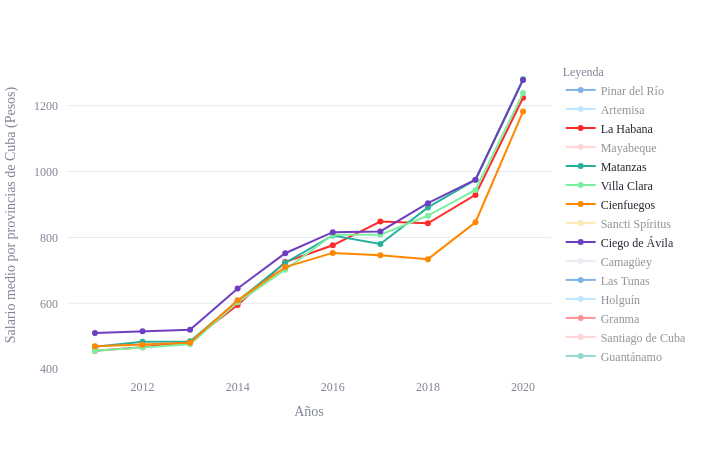
\includegraphics[width=1.0\textwidth]{img/fig6.png}
\end{center}
De igual forma se puede decir, si consideramos las diferencias intermunicipales, que se mantienen con ligera superioridad general los valores de media salarial para la cabeza del municipio, resaltando una vez más el desblanace estructural de distribución de recursos municipales existente en dicho territorio.
\begin{center}
    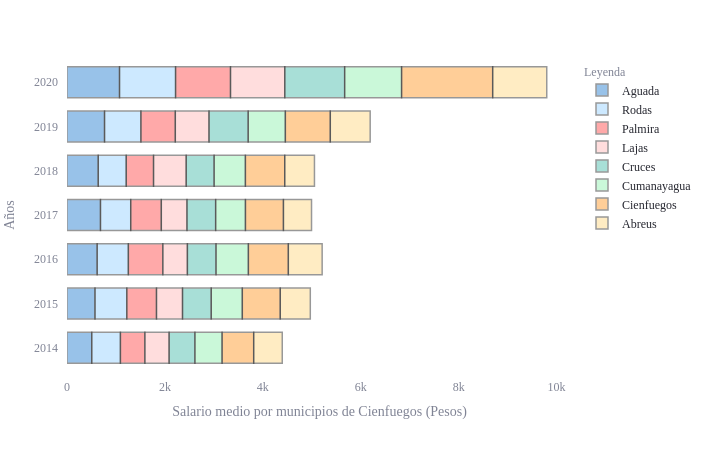
\includegraphics[width=0.8\textwidth]{img/fig7.png}
\end{center}
\emph{\textcolor{blue}{Cabe mencionar que aunque ciertamente esta representación a priori puede que no presente un caracter visualmente significativo, se considera emplear este recurso y la interactividad del mismo para aprovechar el formato de pila barras y reflejar las diferencias de cada municipio con respecto al resto (y de forma general también el desarrollo anual del salario medio del municipio entre los considerados).}}
\clearpage
\section{Encuesta}
Con el objetivo de recopilar perspectivas sobre el tema en cuestión, se llevó a cabo una encuesta online utilizando la aplicación forms.app, la cual fue realizada por 45 personas. Aunque es importante señalar que los resultados de esta encuesta no poseen valor estadístico general debido a su carácter no representativo, no obstante la cantidad de participantes y la estructura intuitiva del cuestionario fomentaron interacciones valiosas y significativas.\\\\
La encuesta fue diseñada para facilitar la participación y animar a los encuestados a compartir sus opiniones, lo que permitió obtener una variedad de respuestas que enriquecen el análisis del tema. A pesar de no ser un conjunto de datos estadísticamente válido, la diversidad de voces y experiencias recogidas brinda un panorama interesante que puede ser considerado para profundizar en la discusión.\\
\begin{itemize}
    \item El desarrollo del formulario planteado sigue el siguiente flujo: \url{https://github.com/LFrench03/La-Perla-del-Sur/tree/main/app/form}
    \item Para ver más detalles (audiencia, respuestas y opiniones) ver en la web: \url{https://la-perla-del-sur.streamlit.app/}
\end{itemize}

\section{Conclusiones y recomendaciones}
En conclusión, el estudio de los procesos migratorios en \textcolor{blue}{Cienfuegos} es crucial para comprender las dinámicas de movilidad poblacional y sus repercusiones socioeconómicas. Las observaciones revelan que la migración hacia la cabecera municipal está motivada por factores como la búsqueda de empleo, acceso a servicios y mayores oportunidades educativas. Sin embargo, esta concentración demográfica también genera desafíos en términos de infraestructura y sostenibilidad. Se recomienda implementar políticas que no solo fortalezcan la infraestructura de la cabecera, sino que también promuevan el desarrollo de las áreas periféricas, garantizando la equidad en el acceso a recursos y oportunidades. Asimismo, es esencial establecer mecanismos de monitoreo para evaluar continuamente el impacto de la migración y ajustar las estrategias en función de las necesidades cambiantes de la población.

\end{document}
